\chapter{Voice-Controlled Lights}

The Internet Of things (IoT) is a field concerned with controlling home appliances using verbal commands. In this project, we will control an array of 3 LEDs using verbal commands by exploiting Bluetooth connectivity.

\subsection*{Components}
\begin{table}[H]
    \centering
    \begin{tabular}{|c|l|c|}\hline
     \textbf{\#} & \textbf{Components} &  \textbf{Amount}\\\hline
     1 & LEDs                       & 3 \\\hline
     2 & 470 $\Omega$ resistors     & 3 \\\hline
     3 & Arduino UNO                & 1 \\\hline
     4 & HC-05: Bluetooth module    & 1 \\\hline
     5 & Connecting wires           & - \\\hline
    \end{tabular}
\end{table}

\subsection*{Connections}

\begin{enumerate}[leftmargin=*]
    \item Connect 470 $\Omega$ resistors with the anode of all LEDs. 
    \item Connect the other end of resistors with pin 4, 5 and 6 of Arduino respectively.
    \item Connect the cathode of all LEDs to GND of Arduino.
    \item Connect Vcc and GND pin of the Bluetooth module with 5V and GND pin on Arduino respectively. 
    \item Connect Tx and Rx pin of the Bluetooth module with Rx and Tx pin of Arduino respectively. 
\end{enumerate}

Fig. \ref{fig:voice} illlustrates the connection of these components.

	\begin{figure}[!ht]
	\centering 
	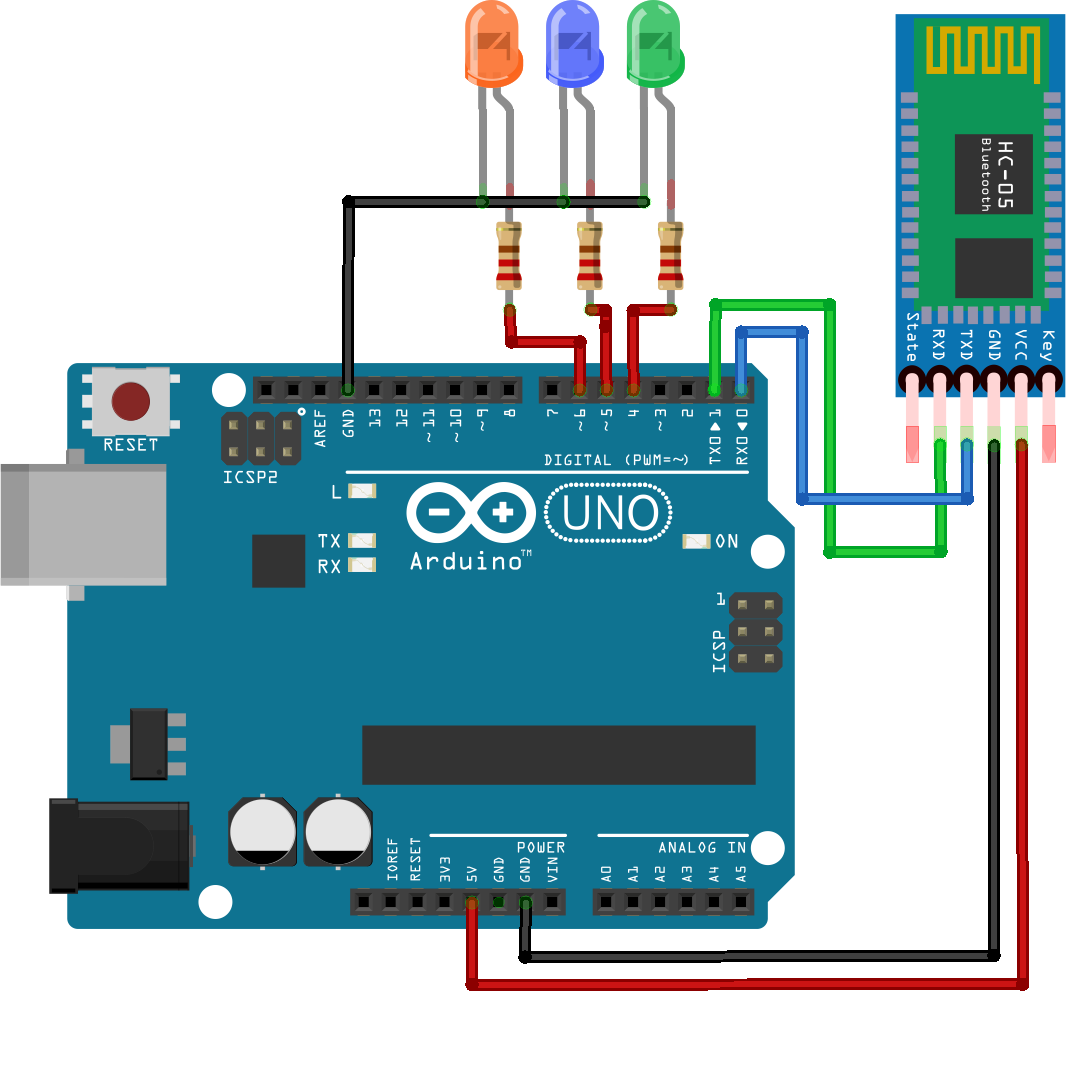
\includegraphics[width=0.4\linewidth]{Figures/recreational_exp/led voice control_bb.png}
	\caption{Circuit diagram of LED controlled using voice commands}
	\label{fig:voice}
	\end{figure}
	
\subsection*{Procedure}

\begin{enumerate}[leftmargin=*]
    \item Copy lst. \ref{list:bluetooth-car} to a new Arduino sketchbook. Upload the code to your Arduino board. Remove Tx and Rx pins of the Bluetooth module while uploading the code.
    \item Turn the switch ON to supply the power to the motor.
    \item Download the app `Arduino Bluetooth RC Car' in your cellphone. 
    \item Turn on Bluetooth of your mobile. Pair with the Bluetooth module by using the default password `1234'. Now open the downloaded app and connect it with the Bluetooth module.  
    \item Select `Voice Control' from the homepage of the app. After that, set letters to be sent for each voice command according to the following table:
    \begin{table}[H]
        \centering
        \begin{tabular}{c|c|c}\hline
            \textbf{LED} &   \textbf{State} & \textbf{Command}\\\hline
            \multirow{2}{*}{1}   &   ON  & A \\\cline{2-3}
                                    &   OFF & B \\\hline
            \multirow{2}{*}{2}   &   ON  & C \\\cline{2-3}
                                    &   OFF & D \\\hline
            \multirow{2}{*}{3}   &   ON  & E \\\cline{2-3}
                                    &   OFF & F \\\hline
        \end{tabular}
    \end{table}
    \item Control the LEDs using dedicated voice commands.
\end{enumerate}
	
\begin{lstlisting}[language=Arduino, numbers=none, caption={Code for LED voice control}, captionpos=b, label={list:led-voice-control}]
// Bluettoth Application to be used: Arduino Bluetooth Control
//vLED pins  
int LED1 = 4;
int LED2 = 5;
int LED3 = 6;

// variable to read data from Bluetooth 
char input; // controlling character

void setup() {
  // put your setup code here, to run once:
Serial.begin(9600);
pinMode(LED1, OUTPUT);
pinMode(LED2, OUTPUT);
pinMode(LED3, OUTPUT);
}

void loop() {
  // put your main code here, to run repeatedly:
    if(Serial.available()>0){
    input= Serial.read();
    Serial.println(input);

// characters to be sent against vocal commands should be configured from the application

//LED1
    if (input= 'A')
    {
      digitalWrite(LED1, HIGH);
    }
     if (input= 'B')
    {
      digitalWrite(LED1, LOW);
    }

//LED2
    if (input= 'C')
    {
      digitalWrite(LED2, HIGH);
    }
     if (input= 'D')
    {
      digitalWrite(LED2, LOW);
    }

  //LED3
    if (input= 'E')
    {
      digitalWrite(LED3, HIGH);
    }
     if (input= 'F')
    {
      digitalWrite(LED3, LOW);
    }
  }
}
\end{lstlisting}

\subsection*{Precautions}
\begin{itemize}[leftmargin=*] 
    \item Do not forget to remove Tx and Rx pins of the Bluetooth module from the Arduino board while uploading the code.
    \item If multiple Bluetooth modules are present at the location, it may create problem in connecting with the required Bluetooth module because all Bluetooth modules have the same password by default. To resolve this issue, AT mode of the Bluetooth module can be used.
    \item If the car is not moving according to the transmitted commands, try swapping the control pins of the motor driver.
\end{itemize}

\begin{figure}[H]
	\centering 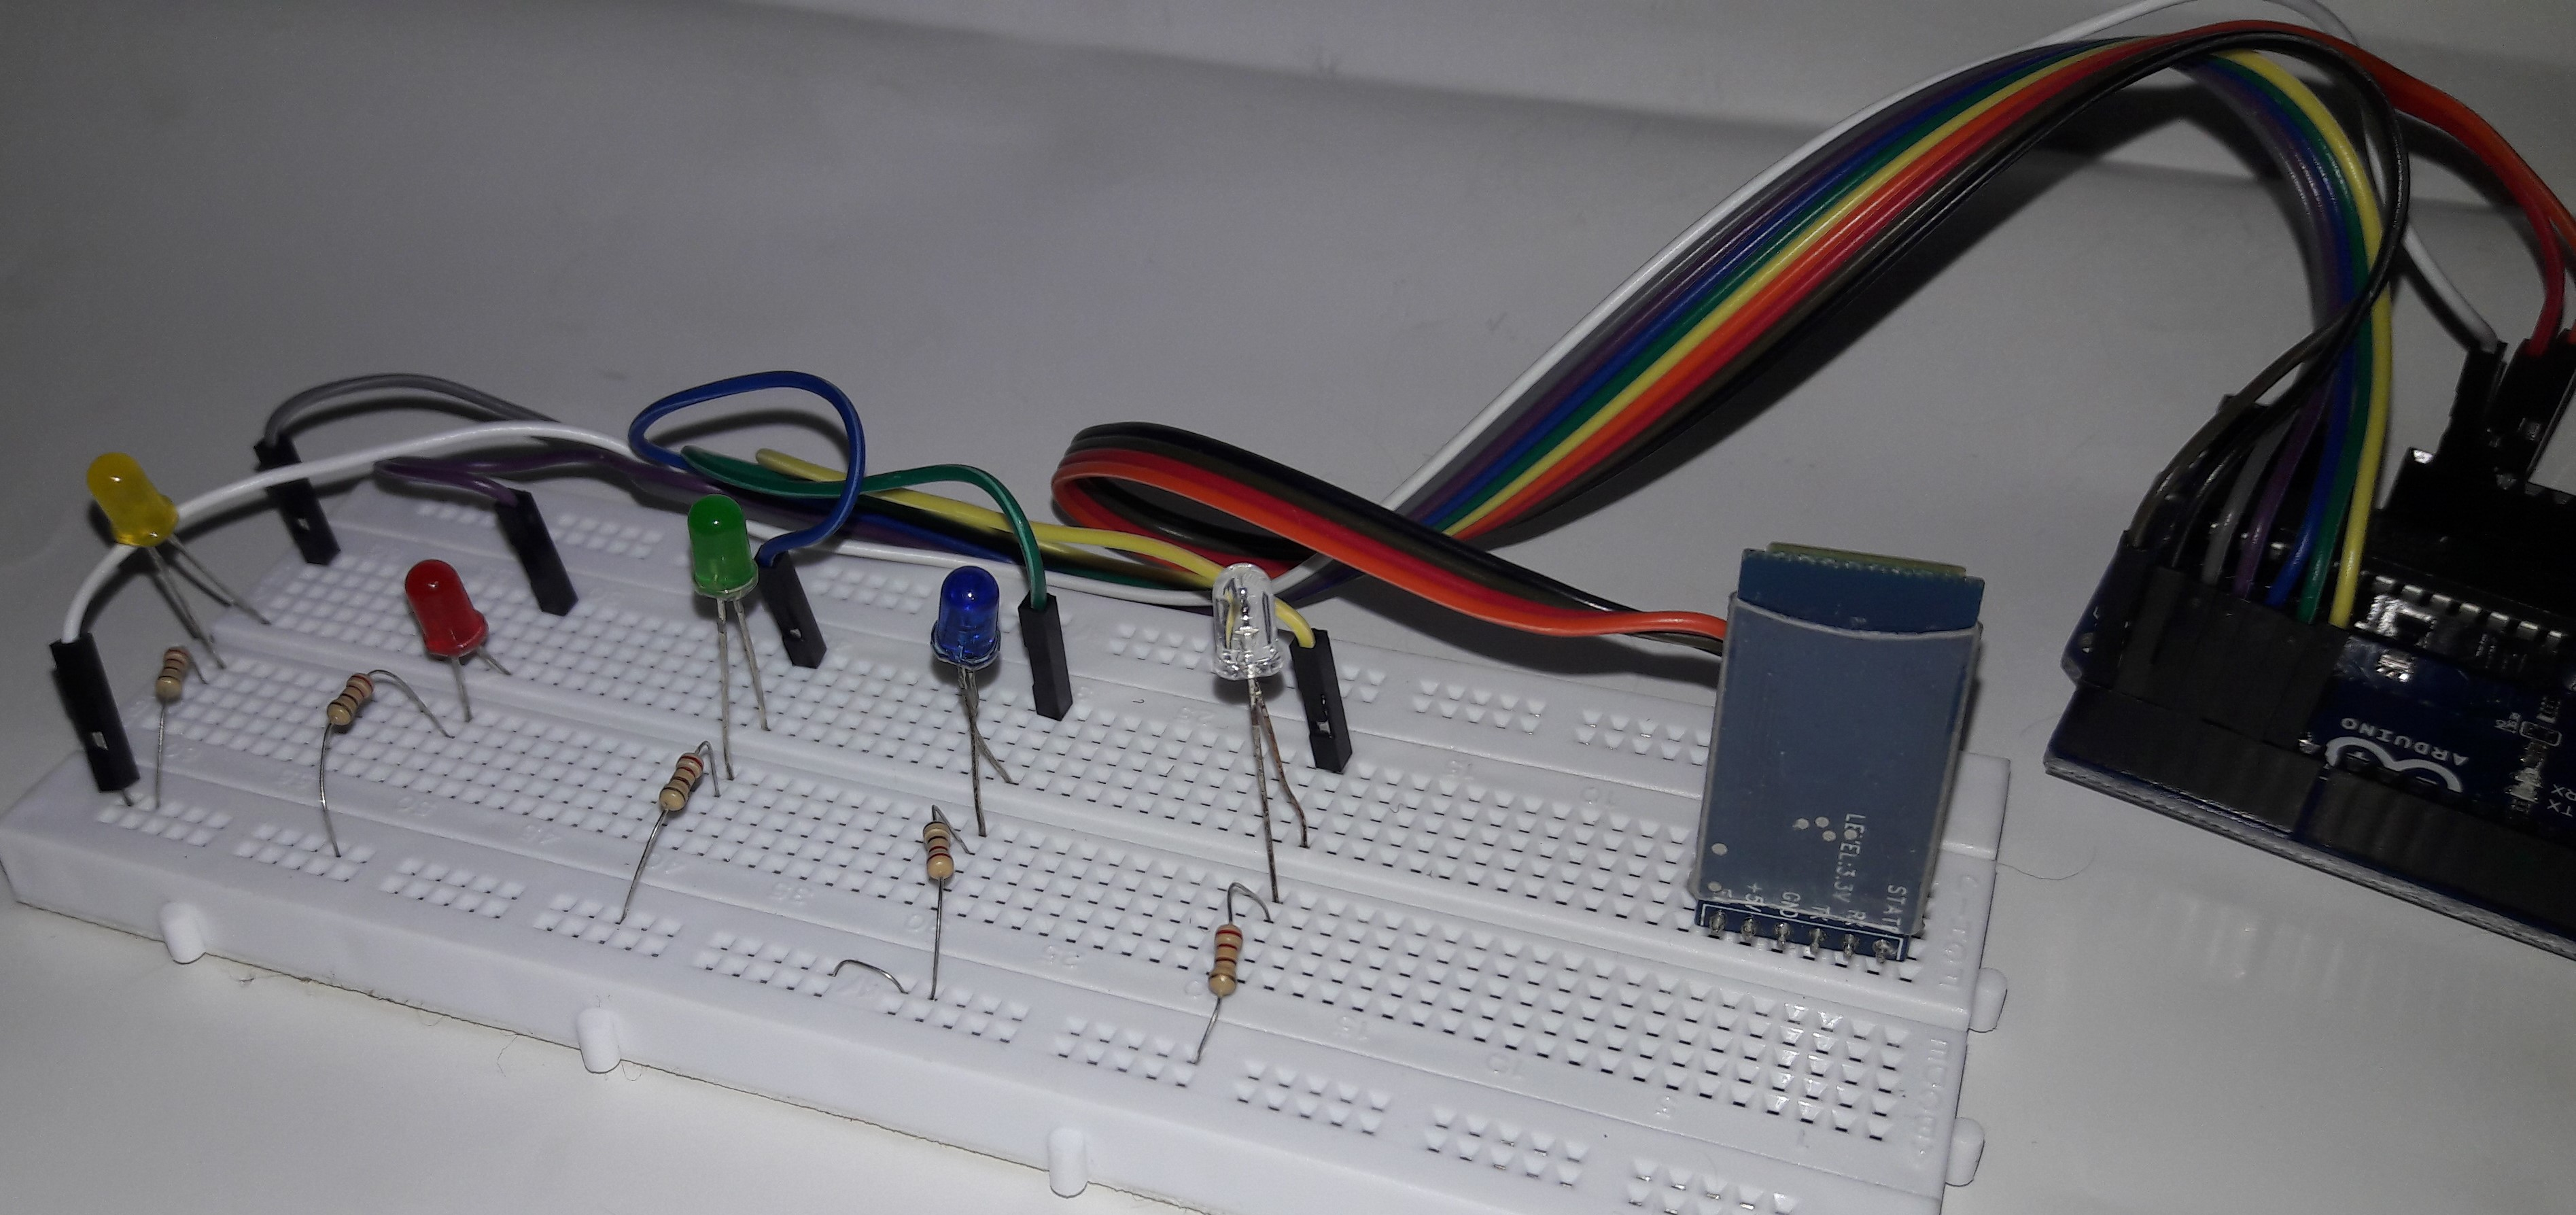
\includegraphics[width=0.7\linewidth]{Figures/recreational_exp/experiment_pics/led voice control.jpg}
	\caption{Hardware of the experiment}
\end{figure}